\documentclass[12pt, a4paper]{report}
\usepackage[top=1cm, left=1cm, right=1cm]{geometry}

\usepackage[utf8]{inputenc}
\usepackage[russian]{babel}

\usepackage{array}
\newcolumntype{M}[1]{>{\centering\arraybackslash}m{#1}}

\usepackage{hyperref}
\hypersetup{
	colorlinks,
	citecolor=black,
	filecolor=black,
	linkcolor=black,
	urlcolor=black
}

\usepackage{sectsty}
\allsectionsfont{\centering}

\usepackage{indentfirst}
\setlength\parindent{24pt}

\usepackage{makecell}

\usepackage{amsmath}

\usepackage{tikz}
\usetikzlibrary{shapes.geometric, arrows}
\usetikzlibrary{arrows.meta}
\usetikzlibrary{decorations.text}

\usepackage{listings}
\usepackage{xcolor}
\definecolor{codegreen}{rgb}{0,0.6,0}
\definecolor{codegray}{rgb}{0.5,0.5,0.5}
\definecolor{codepurple}{rgb}{0.58,0,0.82}
\definecolor{backcolour}{rgb}{0.95,0.95,0.92}
\lstdefinestyle{mystyle}{
    backgroundcolor=\color{backcolour},
    commentstyle=\color{codegreen},
    keywordstyle=\color{magenta},
    numberstyle=\normalsize\color{codegray},
    stringstyle=\color{codepurple},
    basicstyle=\ttfamily\footnotesize,
    breakatwhitespace=false,
    breaklines=true,
    captionpos=b,
    keepspaces=true,
    numbers=left,
    numbersep=5pt,
    showspaces=false,
    showstringspaces=false,
    showtabs=false,
    tabsize=2
}

\usepackage{graphicx}
\graphicspath{ {plots/pictures/} }

\usepackage{booktabs}
\usepackage{csvsimple}
\usepackage{longtable}
\usepackage{caption}

\begin{document}
	\begin{titlepage}
		\begin{center}
			\large \textbf{Министерство науки и высшего образования Российской Федерации} \\
			\large \textbf{Федеральное государственное бюджетное образовательное учреждение высшего образования} \\
			\large \textbf{«Российский химико-технологический университет имени Д.И. Менделеева»} \\

			\vspace*{4cm}
			\LARGE \textbf{ОТЧЕТ ПО ЛАБОРАТОРНОЙ РАБОТЕ №3}

			\vspace*{1cm}
			\LARGE \textbf{Вариант 22}

			\vspace*{4cm}
			\begin{flushright}
				\Large
				\begin{tabular}{>{\raggedleft\arraybackslash}p{9cm} p{10cm}}
					Выполнил студент группы КС-36: & Золотухин А.А. \\
					Ссылка на репозиторий: & https://github.com/ \\
					& CorgiPuppy/ \\
					& num-methods-eq-math-phys-chem-labs \\
					Принял: & Лебедев Данила Александрович \\
					Дата сдачи: & 11.04.2025 \\
				\end{tabular}
			\end{flushright}

			\vspace*{4cm}
			\Large \textbf{Москва \\ 2025}
		\end{center}
	\end{titlepage}

	\tableofcontents
	\thispagestyle{empty}
	\newpage

	\pagenumbering{arabic}

	\section*{Описание задачи}
	\addcontentsline{toc}{section}{Описание задачи}
	\large
	\begin{center}
		\begin{tabular}{||c|c|c|c||}
			\hline
			Вариант & Уравнение & Интервалы переменных & Начальные и граничные условия \\
			\hline
			22 & $ \frac{\partial u}{\partial t}-2\frac{\partial u}{\partial x}=x$ & \makecell{$ x \in [0, 1] $ \\ $ t \in [0, 1] $} & \makecell{$ u(t = 0, x) = 0 $ \\ $ u(t, x = 0) = t^2 $ \\ $ u(t, x = 1) = t^2+t $} \\

			\hline
		\end{tabular}
	\end{center}
	\par
	Для заданного уравнения:
	\begin{enumerate}
		\item записать неявную разностную схему;
		\item определить порядок аппроксимации разностной схемы;
		\item доказать абсолютную устойчивость разностной схемы (с помощью метода гармоник);
		\item вывести рекуррентное соотношение;
		\item выбор граничного условия зависит от того, с какой конечной разностью вы будете работать (левой или правой). Выбор конечной разности зависит от устойчивости системы. Вы должны выбрать ту конечную разность, при которой схема будет устойчива;
		\item составить алгоритм (блок-схему) расчёта;
		\item построить программу на любом удобном языке программирования;
		\item провести численный расчёт с использованием значений $ \Delta t = 0.1 $, $ h = 0.1 $;
		\item сравнить результаты расчётов с истинными значениями функции \textit{u} в соответствующих точках разностной сетки (\textit{истинное} \textit{решение} \textit{уравнения} \textit{будет} \textit{выдано} \textit{преподавателем} \textit{после} \textit{выполнения} \textit{расчётов} \textit{по} \textit{разностной} \textit{схеме});
		\item в случае существенного расхождения результатов расчётов по разностной схеме и истинных значений функции \textit{u} в соответствующих точках разностной сетки выполнить расчёт с меньшими значениями $ \Delta t $ и/или $ h $ (\textit{выбор} \textit{осуществить} \textit{самостоятельно}) с целью получения более точных результатов.
	\end{enumerate}
	\newpage

	\section*{Выполнение задачи}
	\addcontentsline{toc}{section}{Выполнение задачи}

	\subsection*{Задание 1}
	\addcontentsline{toc}{subsection}{Задание 1}
	\large
	Записать неявную разностную схему:
	\begin{equation}\label{eq:implicit}
		\frac{u_{j}^{n+1}-u_{j}^{n}}{\Delta t}-2\frac{u_{j+1}^{n+1}-u_{j}^{n+1}}{h}=(j-1)h.
	\end{equation}
	\par
	В записанной разностной схеме \eqref{eq:implicit} аппроксимация производной функции \textit{u(t, x)} по координате рассматривается на \textit{n+1}-м шаге по времени. Такая разностная схема называется \textbf{неявной}.

	\subsection*{Задание 2}
	\addcontentsline{toc}{subsection}{Задание 2}
	\large
	Определить порядок аппроксимации разностной схемы \eqref{eq:implicit}: \par

	\subsection*{Задание 3}
	\addcontentsline{toc}{subsection}{Задание 3}
	\large
	Доказать абсолютную устойчивость разностной схемы \eqref{eq:implicit} (с помощью метода гармоник): \par
	Для этого отбрасываю член $f(t^{n}, x_{j})$, т.е. $x$ в моём случае, наличие которого не оказывает влияния на устойчивость разностной схемы. \par
	Представлю решение разностной схемы в виде гармоники:
	\begin{equation}\label{eq:harmonic}
		u_{j}^{n} = \lambda^{n}e^{i \alpha j}.
	\end{equation}
	\par
	Подставляя \eqref{eq:harmonic} в разностную схему \eqref{eq:implicit}, получаю:
	\begin{equation*}
		\frac{\lambda^{n+1}e^{i \alpha j} - \lambda^{n}e^{i \alpha j}}{\Delta t} - \frac{\lambda^{n+1}e^{i \alpha (j+1)} - \lambda^{n+1}e^{i \alpha j}}{h} = 0.
	\end{equation*}
	\par
	Упрощаю полученное выражение, деля левую и правую его части на $\lambda^{n}e^{i \alpha j)}$, и выражаю величину, обратную $\lambda$:
	\begin{equation*}
		\frac{\lambda - 1}{\Delta t} - 2\frac{\lambda e^{i \alpha} - \lambda}{h} = 0 \Rightarrow \frac{1}{\lambda} = 1 + 2\frac{\Delta t}{h} - 2\frac{\Delta t}{h}e^{i \alpha}.
	\end{equation*}
	\par
	Необходимое условие устойчивости разностных схем:
	\begin{equation}\label{eq:stability}
		\lvert \lambda \rvert \leq 1.
	\end{equation}
	\par
	При этом необходимое условие устойчивости разностных схем \eqref{eq:stability} также преобразую к виду:
	\begin{equation}\label{eq:reversestability}
		\lvert \frac{1}{\lambda} \rvert \geq 1.
	\end{equation}
	\par
	Неравенство \eqref{eq:reversestability} в применении к комплексным числам означает, что для устойчивости разностной схемы \eqref{eq:implicit} требуется, чтобы величины, обратные собственным числам оператора перехода, были расположены вне или на границе круга радиусом \textit{1}, центр которого находится в начале координат комплексной плоскости (рис. \ref{fig:stability}).
	\begin{figure}
		\centering
		\begin{tikzpicture}[scale=1.6]
			\draw (-3, 0) -- (3, 0) node[right] {Re};
			\draw (0, -3) -- (0, 3) node[above] {Im};
			\foreach \x/\xtext in {-2, -1, 1, 2}
			\draw (\x cm,1pt) -- (\x cm,-1pt) node[anchor=north,fill=none] {$\xtext$};
			\foreach \y/\ytext in {-2/-2i, -1/-i, 1/i, 2/2i}
			\draw (1pt,\y cm) -- (-1pt,\y cm) node[anchor=east,fill=none] {$\ytext$};
			
			\draw (0,0) circle [radius=1cm];
			\draw[postaction={decorate,
				decoration={raise=4pt, text along path,
				text align=center,
				text={1}}}, thick, -Stealth] (0,0) -- (0.7,0.7);
		\end{tikzpicture}
		\caption{Графическая интерпретация условия устойчивости \eqref{eq:stability}}
		\label{fig:stability}
	\end{figure}
	\par
	Введу следующее обозначение:
	\begin{equation*}
		r = 2\frac{\Delta t}{h} > 0 \Rightarrow \frac{1}{\lambda} = 1 + r - re^{i \alpha}.
	\end{equation*}
	\par
	Полученное выражение свидетельствует о том, что собственные числа оператора расположены на комплексной плоскости на окружности с центром в точке $(1 - r,0)$ и радиусом:
	\begin{equation}
		\lvert re^{i \alpha} \rvert = \lvert r\cos{\alpha}+ir\sin{\alpha} \rvert = \sqrt{r^{2}\cos^{2}{\alpha}+r^{2}\sin^{2}{\alpha}} = r.
	\end{equation}
	\par
	Данная окружность находится вне круга, соответствующего условию \eqref{eq:reversestability} при любом значение $r$ (рис. \ref{fig:implicit}). Таким образом, разностная схема \eqref{eq:implicit} будет \textbf{абсолютно устойчива}.
	\begin{figure}
		\centering
		\begin{tikzpicture}[scale=1.6]
			\draw (-3, 0) -- (3, 0) node[right] {Re};
			\draw (0, -3) -- (0, 3) node[above] {Im};
			\foreach \x/\xtext in {-2, -1, 1, 2}
			\draw (\x cm,1pt) -- (\x cm,-1pt) node[anchor=north,fill=none] {$\xtext$};
			\foreach \y/\ytext in {-2/-2i, -1/-i, 1/i, 2/2i}
			\draw (1pt,\y cm) -- (-1pt,\y cm) node[anchor=east,fill=none] {$\ytext$};
			
			\draw (0,0) circle [radius=1cm];
			\draw[postaction={decorate,
				decoration={raise=4pt, text along path,
				text align=center,
				text={1}}}, thick, -Stealth] (0,0) -- (0.7,0.7);
			\draw [blue, very thick] (1+0.4,0) circle [radius=0.4cm];
			\filldraw [black] (1+0.4,0) circle [radius=0.5mm];
			\draw[postaction={decorate,
				decoration={raise=4pt, text along path,
				text align=center,
				text={r}}}, thick, -Stealth] (1+0.4,0) -- (1+0.5,0.4);
		\end{tikzpicture}
		\caption{Исследование устойчивости разностной схемы \eqref{eq:implicit}}
		\label{fig:implicit}
	\end{figure}

	\newpage

	\subsection*{Задание 4}
	\addcontentsline{toc}{subsection}{Задание 4}
	\large
	Вывести рекуррентное соотношение:\par
	Выражая $u_{j}^{n+1}$ из разностной схемы \eqref{eq:implicit}, получаю \textbf{рекуррентное} \textbf{соотношение}
	\begin{equation}\label{eq:recurrent}
		u_{j}^{n+1} = \frac{u_{j}^{n} + 2\frac{\Delta t}{h}u_{j+1}^{n+1} + \Delta t((j - 1)h)}{1 + 2\frac{\Delta t}{h}},
	\end{equation}

	\subsection*{Задание 5}
	\addcontentsline{toc}{subsection}{Задание 5}
	\large
	Выбор граничного условия зависит от того, с какой конечной разностью вы будете работать (левой или правой). Выбор конечной разности зависит от устойчивости системы. Вы должны выбрать ту конечную разность, при которой схема будет устойчива: \par
	Рекуррентное соотношение \eqref{eq:recurrent} позволяет последовательно рассчитать все значения функции \textit{u(t, x)} на \textit{n + 1}-м шаге по времени $u_{j}^{n+1}$, $j = N - 1, \dots, 1$, если известна величина $u_{N}^{n+1}$, которую можно определить из \textit{правого} \textit{граничного} \textit{условия}:
	\begin{equation*}
		u_{N}^{n+1} = ((n + 1)\Delta t)^2 + (n + 1)\Delta t.
	\end{equation*}

	\subsection*{Задание 6}
	\addcontentsline{toc}{subsection}{Задание 6}
	\large
	Составить алгоритм (блок-схему) расчёта:
	\tikzstyle{start} = [circle, draw=black!60, fill=white!5, very thick, minimum size=13mm]
	\tikzstyle{stop} = [circle, draw=black!60, fill=white!5, very thick, minimum size=13mm]
	\tikzstyle{process} = [rectangle, minimum width=3cm, minimum height=1cm, text centered, draw=black]
	\tikzstyle{decision} = [diamond, minimum width=3cm, minimum height=1cm, text centered, draw=black]
	\tikzstyle{arrow} = [thick,->,>=stealth]
	\begin{center}
		\begin{tikzpicture}[node distance=2cm]
			\node (start) [start] {Start};
			\node (in1) [process, below of=start, yshift=-0.5cm] {\makecell{Задание начальных условий: \\ цикл по $j=1..N_{x}$ \\ $u_{j}^{0} = 0$}};
			\node (in2) [process, below of=in1] {$n = 0$};
			\node (dec) [decision, below of=in2, yshift=-1cm] {$n = N_{t}$};
			\node (stop) [stop, right of=dec, xshift=2cm] {End};
			\node (pr1) [process, below of=dec, yshift=-1cm] {\makecell{Определение $u_{N_{x}}^{n+1}$ из граничного условия \\ $u_{N_{x}}^{n+1} = ((n + 1)\Delta t)^2 + (n + 1)\Delta t.$}};
			\node (pr2) [process, below of=pr1, yshift=-0.5cm] {\makecell{цикл по $j=N_{x}-1..1$ \\ $u_{j}^{n+1} = \frac{u_{j}^{n} + 2\frac{\Delta t}{h}u_{j+1}^{n+1} + \Delta t((j - 1)h)}{1 + 2\frac{\Delta t}{h}}$}};
			\node (pr3) [process, below of=pr2, yshift=-0.5cm] {$n = n + 1$};
			\draw [arrow] (start) -- (in1);
			\draw [arrow] (in1) -- (in2);
			\draw [arrow] (in2) -- (dec);
			\draw [arrow] (dec) -- node[anchor=south] {да} (stop);
			\draw [arrow] (dec) -- node[anchor=west] {нет} (pr1);
			\draw [arrow] (pr1) -- (pr2);
			\draw [arrow] (pr2) -- (pr3);
			\draw [arrow] (pr3.west) -- ++(left:5cm) -| +(up:8cm) -- (dec.west);
		\end{tikzpicture}
	\end{center}	

	\subsection*{Задание 7}
	\addcontentsline{toc}{subsection}{Задание 7}
	\large
	Построить программу на любом удобном языке программирования:
	\lstset{style=mystyle}
	\lstinputlisting[language=C++]{src/main.cpp}

	\subsection*{Задание 8}
	\addcontentsline{toc}{subsection}{Задание 8}
	\large
	Провести численный расчёт с использованием значений $ \Delta t = 0.1$, $ h = 0.1 $:
	\begin{center}
	\small
	\captionof{table}{Результаты для $\Delta t = 0.1$}
	\label{tab:results_01}
		\begin{longtable}{|c|c|c|c|c|c|c|c|c|c|c|c|}
		\hline
		$t \backslash x$ & 0 & 0.1 & 0.2 & 0.3 & 0.4 & 0.5 & 0.6 & 0.7 & 0.8 & 0.9 & 1 \\\hline
		\endfirsthead

		\hline
		$t \backslash x$ & 0 & 0.1 & 0.2 & 0.3 & 0.4 & 0.5 & 0.6 & 0.7 & 0.8 & 0.9 & 1 \\\hline
		\endhead

		\endfoot
		\endlastfoot

		\csvreader[
		  late after line=\\,
		  late after last line=\\\hline\multicolumn{12}{c}{},
		  head to column names,
		  respect all
		]{outputs/output_0.1.csv}{}{
		  \csvcoli & \csvcolii & \csvcoliii & \csvcoliv & \csvcolv & \csvcolvi & \csvcolvii & \csvcolviii & \csvcolix & \csvcolx & \csvcolxi & \csvcolxii
		}
		\end{longtable}
	\end{center}

	\subsection*{Задание 9}
	\addcontentsline{toc}{subsection}{Задание 9}
	\large
	Составить отчёт о проделанной работе. График функции \textit{u(t, x)}
	\begin{center}
		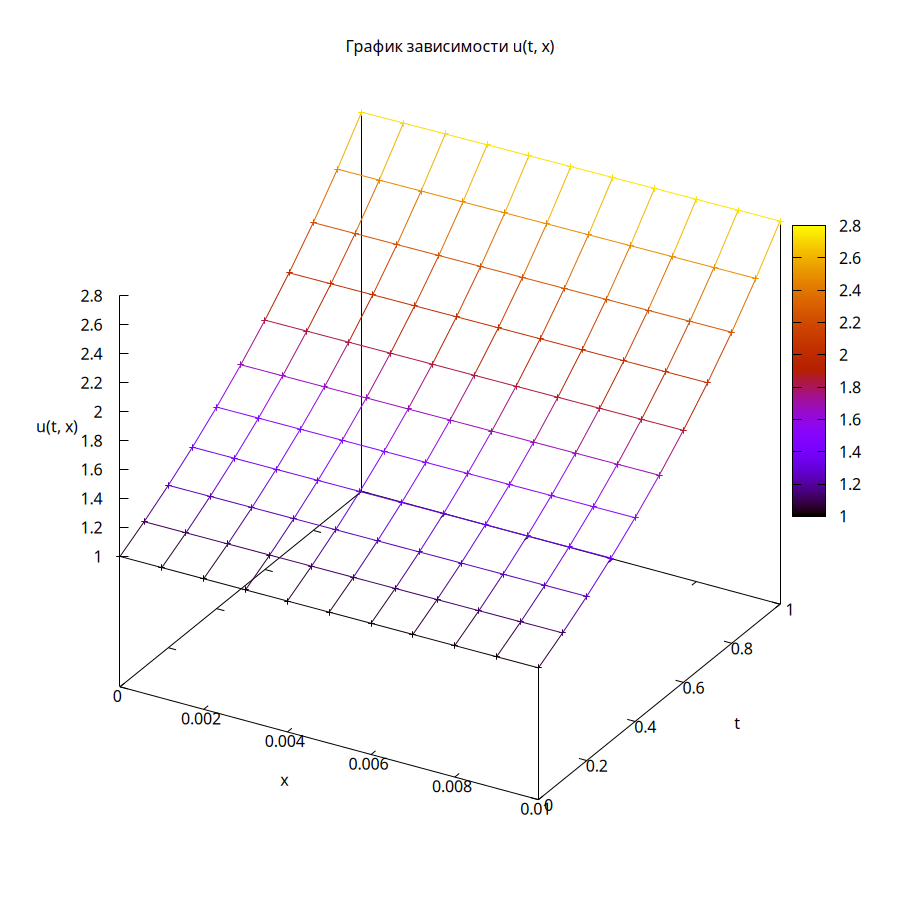
\includegraphics[width=500pt]{u_t_x_0.1.png}
	\end{center}
\end{document}
